\documentclass[11pt]{article}

\usepackage[utf8]{inputenc}
\usepackage{geometry}
\usepackage{color,graphicx,framed}
\usepackage{amsmath,amsfonts,amssymb}
\usepackage{listings}
\usepackage[section]{placeins}
\usepackage{pstricks,pst-tree,pst-node}
\usepackage{dsfont}
\usepackage{ulem}
\usepackage{nicefrac}
\usepackage{multirow}

\title{Abschlussbericht\\Proseminar Algorithmen\\Vortrag :Parallele Sortierung}
\author{Patrick Winterstein,Björn Rathjen}
\date{SS14}

\begin{document}
\maketitle
\newpage
\tableofcontents
\newpage
\listoffigures
\listoftables
\section{Einführung}
Der Titel Paralleles Sortieren beschreibt zwei grundsätzliche Bestrebungen bei der Optimierung von Netzwerk- (hauptsächlich Routing) und Datenstrukturen (Listen, Wörterbücher, \dots). Somit ist die Motivation dieses Thema zu behandeln groß, da sie für jene Projekt die Basis für deren Geschwindigkeit legen kann. Separat betrachtet sind diese von folgender Bedeutung :
\begin{description}
\item[Sortierung] Sortierung ist die Basis für jede Suche auf Daten und Ressourcen. Wenn diese nicht wenigstens einer groben Ordnung unterliegen können effiziente Algorithmen nicht angewendet werden, da keine Annahmen über den Zustand getroffen werden können.
\item[Parallelität] Durch den Aufwand von mehr Ressourcen kann ein Sortierprozess beschleunigt werden ohne die Korrektheit des Ergebnisses zu gefährden. Dabei ist Parallelität der Extremfall, der eine Maximierung des Datendurchsatzes erlaubt und somit in einer höheren Geschwindigkeit gegenüber sequentiellen Ansätzen resultiert.
\end{description}
\section{Grundlagen}

\subsection{Sortieren}
Als Grundlage um eine Menge M sortieren zu können muss eine Ordnungsrelation R vorhanden sein, diese schreibt eine Ordnung zwischen zwei Elementen vor. 
\begin{equation}
R \subseteq M \times M
\label{eq:Ordnung}
\end{equation}
Der Anspruch an diese Relation ist, dass diese Transitivität beinhaltet.
\begin{equation}
\forall x,y,z \in M : xRy \wedge yRz \Rightarrow xRz
\label{eq:transit}
\end{equation}
Würde eine dieser Voraussetzungen nicht erfüllt sein, so würde bei \eqref{eq:Ordnung} kein sortieren möglich sein, da keine Relation vorhanden ist, und bei \eqref{eq:transit} die Relation zweier Elemente untereinander keine Aussage über die Relation zu anderen Elementen aussagt. Daraus resultiert das das "sortierte" Ergebnis nur zu einem Element als sortiert betrachtet werden kann.
\subsection{Komparator}
Ein Komparator stellt den kleinsten Baustein dar, der eine zweielementige Menge entsprechend der auf ihr liegenden Ordnungsrelation sortiert ausgibt. Dieser ist wie folgt aufgebaut. Er besitzt zwei Eingangsleitungen auf dem die zu sortierenden 2-elementigen Mengen eingegeben werden, den vergleichenden Teil, der die Ordnungsrelation anwendet und die beiden Ausgangsleitungen, auf denen das sortierte Ergebnis ausgegeben wird. Beide werden in Abbildung \ref{fig:kompsoft} (Software, Seite \pageref{fig:kompsoft})) und Abbildung \ref{fig:komparator} (Hardware, Seite \pageref{fig:komparator}) dargestellt. Die Annahme für die folgenden Abbildungen ist, dass das sortierte Ergebnis von oben nach unten größer wird.
\begin{figure}
\begin{center}
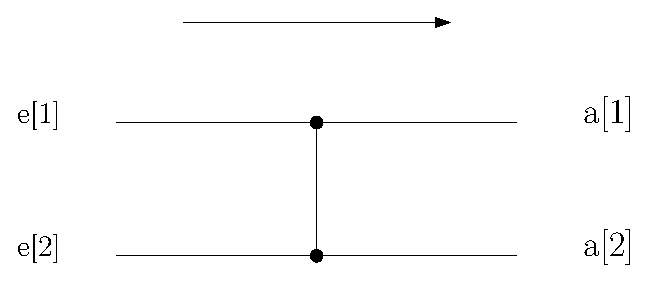
\includegraphics[scale=0.8]{Komparator1.eps}
\end{center}
\caption{Schema eines Komparators. e entspricht den Eingängen und a den Ausgängen. Der Pfeil gibt die Durchlaufrichtung an. Die waagerechten schwarzen Linien entsprechen den Datenleitungen, die senkrechte Linie zeigt die vergleichenden Teil an.}
\label{fig:komparator}
\end{figure}
\begin{figure}
\begin{lstlisting}[language=C,tabsize=4,numbers=left]
    void comp(chan in1, in2, out1, out2 Comparer{}){
        a := <- in1
        b := <- in2
        
        if (a < b){
            out1 <- a
            out2 <- b
            return void
        }
        out1 <- b
        out2 <- a
        return void
    }
\end{lstlisting}
\caption{Implementierung eines Komparators in Pseudocode (An Go angelehnt). inX entspricht den Eingangsleitungen, outX entspricht den Ausgangsleitungen, Comparer besagt, dass der Datentyp die beschriebenen Voraussetzungen (\eqref{eq:Ordnung} und \eqref{eq:transit}) erfüllt. "return void" zeigt, dass die Funktion nur die Ein- und Ausgänge verwendet.}
\label{fig:kompsoft}
\end{figure}
\FloatBarrier
\section{Sortiernetzwerk}
Die im vorherigen Abschnitt beschriebenen Voraussetzungen dienen nun als Grundlage dafür ein größeres Netzwerk aufzubauen, das folgende Eigenschaften besitzt:
\begin{itemize}
\item mehr als 2 Eingabeleitungen
\item Ausgabe soll sortiert sein
\end{itemize}
Das Netzwerk soll zusätzlich nur aus Komperatoren bestehen. Es wird noch kein Anspruch an Komplexität und Effizienz erhoben.
\FloatBarrier
\subsection{Aufbau}
Ein naiver Ansatz für den Aufbau des Netzwerks wird in Abbildung \ref{fig:kompnetsmall}(Seite \pageref{fig:kompnetsmall}) gezeigt. Die Anzahl der Leitungen wurde verdoppelt und die Anzahl der Komparatoren angepasst. In Abbildung \ref{fig:kompnetnumbex} (Seite \pageref{fig:kompnetnumbex}) wird der Vollständigkeit halber ein größeres Zahlenbeispiel gezeigt. Die Sortierung der vorher unsortierten Eingabe kann schrittweise verfolgt und überprüft werden.
\begin{figure}
\begin{center}
\begin{minipage}[l]{2cm}
Input
\end{minipage}
\begin{minipage}[c]{7cm}
\begin{center}
    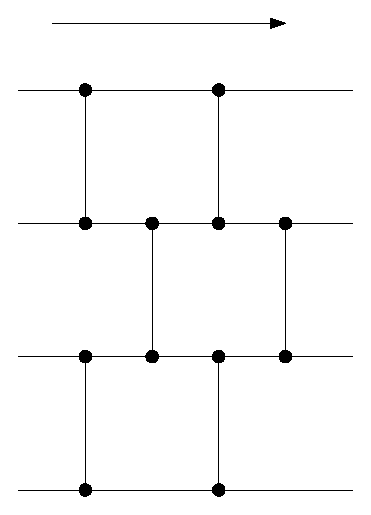
\includegraphics[scale=0.8]{bild2Komparatornetzwerk.eps}
\end{center}
\end{minipage}
\begin{minipage}[r]{2cm}
Output
\end{minipage}
\end{center}
\caption{Komparatornetzwerk mit mehreren Datenleitungen}
\label{fig:kompnetsmall}
\end{figure}
\begin{figure}
\begin{center}
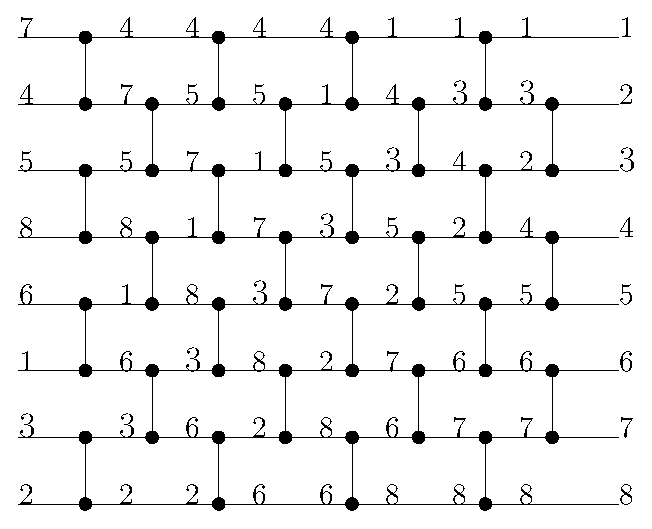
\includegraphics[scale=1]{bild2beispiel.eps}
\caption{Beispiel mit acht Datenleitungen dass einen schrittweisen Verlauf des sortierens zeigt und eine vollständig sortierte Ausgabe.}
\label{fig:kompnetnumbex}
\end{center}
\end{figure}
\FloatBarrier
\subsection{Korrektheit}
\subsubsection{Betrachtung der Analyse}
Problematisch bei der Überprüfung durch Beispiele ist die große Anzahl an der zu überprüfenden Fälle sehr groß ist. Im Beispiel in Abbildung \ref{fig:kompnetnumbex} (Seite \pageref{fig:kompnetnumbex}) bei einer Eingabemenge mit den Elementen 1 bis 8 wären dies 40320 unterschiedliche Fälle (diese Anzahl ist durch den Ausschluss, dass eine Zahl mehrfach vorkommt bereits reduziert worden) Allgemein ist die Anzahl $\nicefrac{n!}{(n-l)!}$, wobei n die möglichen Elemente und l die Anzahl der Datenleitungen ist. Nachfolgend wird nun eine einfachere Möglichkeit gezeigt, wie die Korrektheit überprüft werden kann.
\subsubsection{0,1-Prinzip}
Das 0,1-Prinzip ist ein Werkzeug zur Überprüfung, ob ein Sortiernetzwerk alle Eingaben richtig sortiert. Dabei wird die Menge von Testfällen reduziert, indem man die Eingabemenge auf die Zeichen 0 und 1 beschränkt.
\paragraph{Lemma}
Wenn es eine Folge A gibt, die ein Sor\-tier\-netz\-werk nicht sortiert, so existiert auch eine 0,1-Folge, die von diesem Netzwerk nicht sortiert wird.
\paragraph{Beweis} Geführt wird ein Beweis durch Widerspruch. 
\begin{enumerate}
\item[i)] Annahme : Wenn ein Sortiernetzwerk / Algorithmus eine Eingabe nicht sortiert, so sortiert er trotzdem alle 0,1-Folgen.
\item[ii)] Voraussetzungen : \begin{itemize}
\item Eingabefolge $E = e_0 \dots e_l$
\item sortiere Eingabefolge $ S = s_1 \dots s_l$
\item unsortierte Ausgabefolge von E $ U = u_1 \dots u_l $
\item kleinster Index an dem $u_k \neq s_k$ 
\end{itemize}
\item[iii)] Folgerungen aus ii) :
\begin{eqnarray}
u_i = s_i & & \forall \ i \neq 0 \wedge i < k \\
u_r = s_k & & \text{mit } r > k
\end{eqnarray}
\item[iv)] Funktion, die ein 0,1-Folge aus einer beliebigen anderen Folge erstellt. Die Konstante, die dazu verwendet wird, ist in diesem Fall $s_k$.
\begin{equation}
f(e) = \begin{cases} 0 , & if \;\; e_i \leq s_k \\
    1 , & if \;\; e_i > s_k
    \end{cases}
\label{eq:cases}
\end{equation}
\item[v)] Wendet man die Funktion nun auf die Eingabe / Ausgabe an, so entsteht eine 0,1-Folge der Form 
\begin{equation}
00 \dots 01_k\dots0_r \dots
\label{eq:01folge}
\end{equation}
\item[vi)] Folgerung : \\
$\Rightarrow$ die Folge ist unsortiert.\\
$\Rightarrow$ Widerspruch zur Annahme
\end{enumerate}
\paragraph{Vorteile} Durch das Anwenden des 0,1-Prinzips wird die Anzahl der Testfälle von 
\begin{equation}
n! \rightarrow 2^l
\label{eq:fallred}
\end{equation} 
reduziert. Daraus resultiert ,das mit größerer Sicherheit und effektiver getestet werden kann.
\FloatBarrier
In einem Beispiel in Abbildung \ref{fig:01ex} (Seite \pageref{fig:01ex}) wird die Zuweisung mit $s_k = 6$ demonstriert und die anschließende Sortierung. 
\begin{figure}
\begin{center}
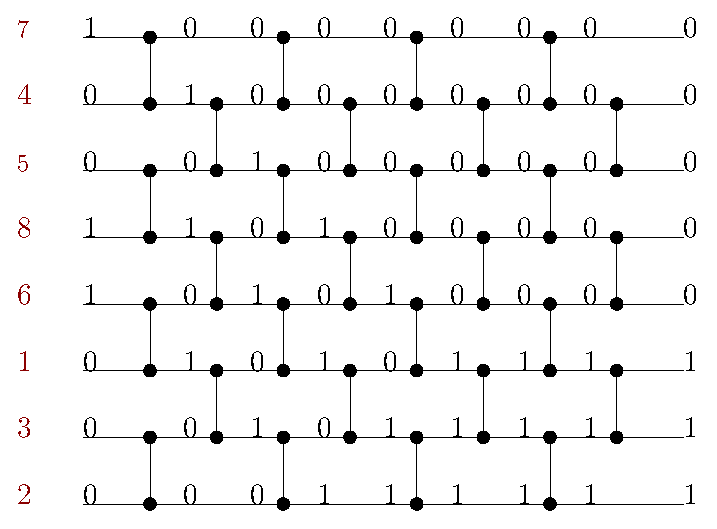
\includegraphics[scale=0.75]{01beispiel.eps}
\end{center}
\caption{Beispiel für das 0,1-Prinzip. Folge wird auf das Beispiel aus Abbildung \ref{fig:kompnetnumbex} (Seite \pageref{fig:kompnetnumbex}) angewendet. Es zeigt, dass das Resultat für die gewählte Konstante sortiert ist. Genauso zeigt es auch das bis Schritt 5 die Folge nicht sortiert ist.}
\label{fig:01ex}
\end{figure}
\subsection{Übertragung von Sortieralgorithmen auf ein Sortiernetzwerk}
\subsubsection{Bubblesort}
\FloatBarrier
Netzwerkimplementierung (Abbildung \ref{fig:bubblesort} Seite \pageref{fig:bubblesort}) entspricht der Softwareimplementierung. Die Datenleitungen entsprechen den Indizes einer Liste von oben nach unten. Die Vergleiche folgen dem Algorithmus, Optimierungen in Form von Parallelen Vergleichen wurden bereits vollzogen.
\begin{figure}
\begin{center}
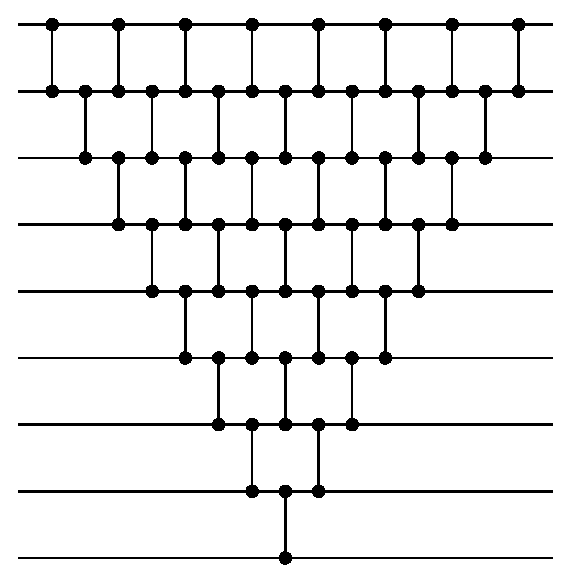
\includegraphics[scale=0.8]{bubblesort.eps}
\end{center}
\caption{Bubblesort: Bubblesort mit parallelen Vergleichen.}
\label{fig:bubblesort}
\end{figure}
\FloatBarrier
\subsubsection{Quicksort , Mergesort}
Bei Versuch schnellere Algorithmen zu implementieren entstehen durch direkte Umwandlung Probleme. 
\begin{description}
\item[Quicksort] Bei Quicksort wird in jedem Schritt ein Pivotelement gewählt nach dem die übrigen Werte auf zwei Listen aufgeteilt werden. Dies stellt in einem starren Netzwerk ein Problem dar, da die Größen dieser Listen von der Eingabe abhängen, und somit nach dem ersten Vergleich die Position des Pivotelemnts nicht mehr festgelegt ist. 
\item[Mergesort] Bei Mergesort wird die Eingabe in maximal 2-elementige Listen unterteilt, der danach dynamische merge-Prozess lässt sich nicht 1:1 auf ein starres Netzwerk übertragen
\end{description}
Dies wird in Abbildung \ref{fig:mergesort} (Seite \pageref{fig:mergesort}) verdeutlicht.
\begin{figure}
\begin{center}
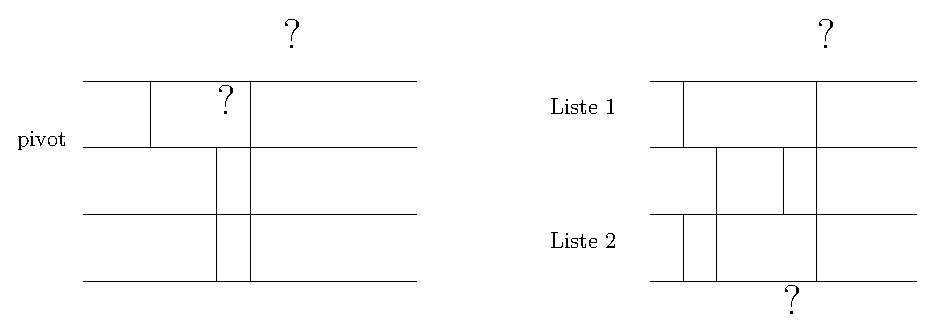
\includegraphics[scale=0.8]{mergesort.eps}
\end{center}
\caption{Auf der linken Seite ist der Versuch Quicksort, auf der rechten Seite Mergesort zu implementieren zu sehen}
\label{fig:mergesort}
\end{figure}
\subsection{Biton-Sortierer}
Der Biton-Sortierer ist ein Sortierverfahren, welches mit dem Teile-und-Hersche-Prinzip eine Menge sortiert.
\subsubsection{Das Verfahren}
Zur Vereinfachung betrachten wir Eingabemengen M der Länge $2^x$.\\
\begin{description}
\item[Schritt 1] Teilen\\Zuerst wird Eingabemenge in die 2 Hälften $m_0, m_1, ..., m_{n/2-1}$ und $m_{n/2}, m_{n/2+1}, ..., m_{n-1}$ aufgeteilt. Diese werden rekursiv mit einem Biton-Sortierer sortiert.
\item[Schritt 2] Herschen\\Vergleiche [$m_i$:$m_{2^x-i}$] i = $\{0, 1, ..., 2^{x-1}\}$\\Solange n $<$ 1:\\ Vergleiche [$m_i$:$m_{n/4+i}$] und [$m_{n/2+i}$:$m_{3n/4+i}$] i = $\{0, 1, ..., 2^{x-2}\}$\\Wiederhole für die Teilmengen $m_0$,$m_1$,...,$m_{n/2}$ und $m_{n/2}$,$m_{n/2+1}$,...,$m_{n}$
In einem Sortiertnetzwerk sieht das Herschen nun wie folgt aus:\\
\begin{center}
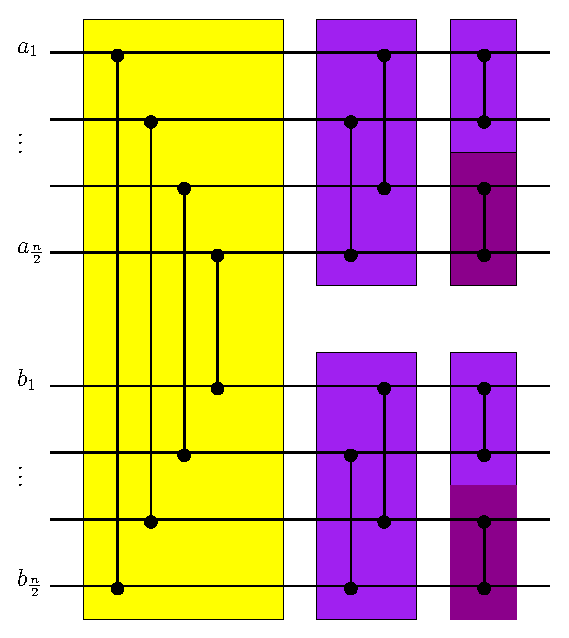
\includegraphics[scale=0.8]{bitonmischer.eps}
\end{center}
\end{description}
\subsubsection{Korrektheit}
Um die Korrektheit des Bitonen-Sortierers zu zeigen, benutzen wir das 0-1 Prinzip und beschränken die Eingabefolge auf 0'en und 1'en.\\
Seien ($a_1$, $a_2$, ..., $a_{n/2}$) und ($b_1$, $b_2$, ..., $b_{n_2}$) die 2 Hälften der Eingabefolge, die beide sortiert sind.
\begin{description}
\item[Schritt 1] Vorsortierung\\Im 1. Schritt werden die kleinereren Elemente nach "oben" und die größeren Elemente nach "unten" sortiert. Bei einer Eingabemenge von \{0, 1\} besteht entweder die "obere" Hälfte nur aus 0'en oder die "untere" Hälfte nur aus 1'en.\\ Die unsortierte Hälfte hat nun die Form 0...01...10...0 ("oben") oder 1...10...01...1 ("unten").
\item[Schritt 2] "Rekursion"\\Im 2. Schritt wird das Prinzip aus dem 1. Schritt für die immer kleiner werden Hälften angewendet, d.h. wir sortieren die kleineren Elemente nach "oben" und die größeren nach "unten".\\
\begin{figure}
\begin{center}
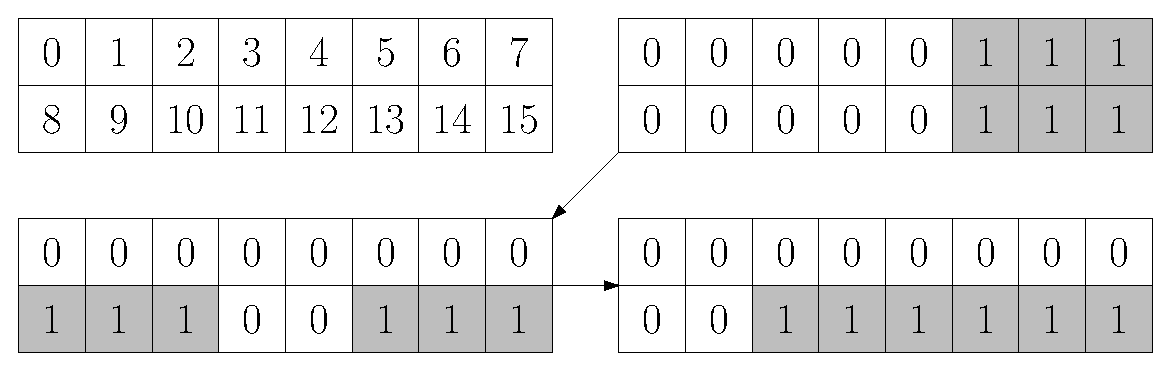
\includegraphics[scale=0.4]{korrektheitBS.eps}
\caption{•}
\end{center}
\end{figure}
\FloatBarrier
Damit ist die Folge sortiert, wenn wir bei 1-elementigen Elementen angekommen sind. 
\end{description}
\subsection{Odd-Even-Mergesort}
Das Odd-Even-Mergesort ist ein Sortierverfahren, welches dem Biton-Sortierer ähnelt. Da es datenunabhängig ist, eignet es sich perfekt für die Umsetzung in ein Sortiernetzwerk.
\subsubsection{Merge-Verfahren}
Das Merge-Verfahren setzt vorraus, dass die beiden Hälften $m_0, m_1, ..., m_{n/2-1}$ und $m_{n/2}, m_{n/2+1}, ..., m_{n-1}$ der Eingabefolge $m_0, m_1, ..., m_n$ soriert sind.
\begin{description}
\item[Wenn n $>$ 2] .\\1. Wende Odd-Even-Mergesort auf die beiden Teilfolgen \\$m_0, m_2, m_4, ..., m_{n-2}$ und \\$m_1, m_3, m_5, ..., m_{n-1}$ an.\\ 2. Vergleiche $m_i$ und $m_{i+1}$ $\forall \; i \in \{1, 3, 5, n-3\}$
\item[sonst].\\Vergleiche $m_0$ und $m_1$
\end{description}
\subsubsection{Sortier-Verfahren}
Das Merge Verfahren setzt sortierte Teillisten vorraus. Dies ist in der Praxis normalerweise nicht gegeben.
Um diese Vorraussetzung zu umgehen, kann man das Odd-Even-Mergesort einfach rekursiv aus die Teillisten anwenden:
\begin{description}
\item[Wenn n $>$ 1].\\1. Wende Odd-Even-Mergesort rekursiv auf beiden Hälften $m_0, m_1, ..., m_{n/2-1}$ und $m_{n/2}, m_{n/2+1}, ..., m_{n-1}$ der Eingabefolge anwenden.\\2. Wende Odd-Even-Merge auf die Eingabefolge M an.
\item[sonst].\\Eingabgefolge bereits sortiert
\end{description}
\subsubsection{Korrektheit}
Um die Korrektheit zu zeigen, beweisen wir das Merge-Verfahren für eine Eingabefolge M mit n Elementen. Die Zeichen der Eingabefolge beschränken wir auf 0 und 1.
\begin{description}
\item[Beweis durch Induktion]
\item[Induktionsanker] n = $2^1$\\ Es wird der Vergleich der "sonst"-Klausul ausgeführt. Damit ist die Folge offensichtlich sortiert.
\item[Induktionsvoraussetzung (IV)] Das Sortierverfahren sei für n = $2^x$ korrekt
\item[Induktionsschritt  $2^x \rightarrow 2^{x+1}$]
In Schritt 1 des Sortierverfahrens wird die Eingabemenge in halbiert und die beiden Hälften mit Odd-Even-Mergesort sortiert. Nach Induktionsvoraussetzung sind die beiden Hälften danach korrekt sortiert. Nun wenden wir das Merge-verfahren auf diese Menge an.\\Um die Korrektheit des Mergeverfahrens zu zeigen, betrachten wir die Anzahl von 1'en und 0'en in den Mengen.\\Zuerst betrachten wir die beiden sortierten Hälften aus Schritt 1. 
\begin{description}
\item[Menge 1:] $|$1'en$|$ sei $n_0$ und $|$0'en$|$ sei $p_0$.
\item[Menge 2:] $|$1'en$|$ sei $n_1$ und $|$0'en$|$ sei $p_1$.
\end{description}
 Wenn wir diese beiden Mengen wieder zusammenfügen und dann in folgende Mengen aufteilen: 
$$M_0 \; = \; m_0, m_2, m_4, ..., m_{n-2}$$ 
$$M_1 \; = \; m_1, m_3, m_5, ..., m_{n-1}$$ 
Werden die 0'en und 1'en "gleichmäßig" aufgeteilt. 
$$M_0 \; :\; | \text{1'en} | \; = \;\left\lfloor \frac{n_0}{2} \right\rfloor + \left\lfloor \frac{n_1}{2} \right\rfloor \text{und $|$0'en$|$} \;=\; \left\lceil \frac{p_0}{2} \right\rceil + \left\lceil \frac{p_1}{2} \right\rceil$$
$$M_1 \;:\; \text{|1'en|}  = \left\lceil \frac{n_0}{2} \right\rceil + \left\lceil \frac{n_1}{2} \right\rceil  \text{und |0'en|} \;=\; \left\lfloor \frac{p_0}{2} \right\rfloor + \left\lfloor \frac{p_1}{2} \right\rfloor$$
Nun betrachten wir die Differenz von $|$1'en$|_{M_0}$ und $|$1'en$|_{M_1}$:
\begin{description}
\item[Fall 1:] Seien $n_0$ und $n_1$ gerade: $|$1'en$|_{M_0}$ = $|$1'en$|_{M_1}$.
\item[Fall 2:] Sei $n_0$ oder $n_1$ ungerade: $|$1'en$|_{M_0}$ = $|$1'en$|_{M_1}$ - 1.
\item[Fall 3:] Seien $n_0$ und $n_1$ ungerade: $|$1'en$|_{M_0}$ = $|$1'en$|_{M_1}$ - 2.
\end{description}
Die beiden Teilmengen $M_0$ und $M_1$ werden nun wieder sortiert (da die Länge wiederrum $2^x$ ist, gilt IV), danach ergibt sich eines der folgenden Schemata:
\end{description}
\begin{figure}[!hb]
\begin{center}
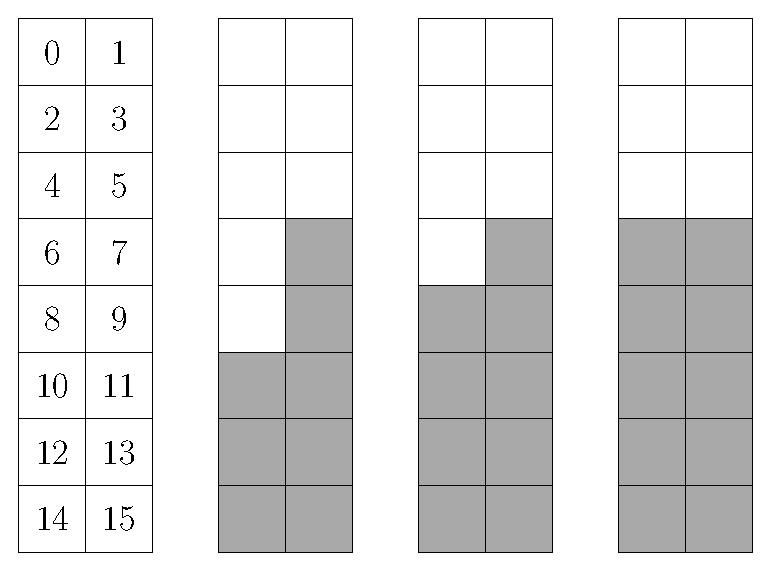
\includegraphics[scale=0.4]{korrektheitOEM.eps}
\caption{• uiae }
\end{center}
\end{figure}
Wenden wir nun Schritt 2 des Mergeverfahrens an, ist die Liste sortiert.
\FloatBarrier
\section{Laufzeit}
Die Laufzeit von parallelen Algorithmen wird durch die Anzahl nacheinander ausgeführten Schritten bestimmt.
\subsection{Herleitung}
Die Laufzeit der beiden vorgestellten Sortieralgorithmen unterscheidet sich in O-Notation nicht, deshalb beschränken wir uns auf die Herleitung an einem Beispiel:\\
\begin{table}[!hb]
\begin{center}
	\begin{tabular}{c | c}
		Länge der Eingabe & Anzahl der Schritte \\ \hline
		$2^1$ & 1 \\
		$2^2$ & 1+2 \\
		$2^k$ & 1+2+3+...+k-1+k \\
		& = $\sum_{i=1}^ki$ = $\frac{1}{2} * log_2n (log_2n +1) $
	\end{tabular}
\end{center}
\caption{Entwicklung der Laufzeit}
\end{table}
Damit ergibt sich eine Laufzeit von O($(log(n))^2$)
\section{Vergleich der Laufzeit}
Um die Laufzeit von parallelen Algorithmen mit der von sequentiellen zu Vergleichen, wir die Anzahl der Schritte in parallelen Algorithmen mit der maximalen Anzahl von Komponenten multipliziert.\\
Damit ergibt sich eine normalisierte Laufzeit von O($n*log^2$) für die vorgestellten parallelen Algorithmen.
\begin{table}[hb]
\begin{center}
	\begin{tabular}{c|c|c|c}
		Algorithmus & \multicolumn{3}{|c}{Laufzeit} \\ \hline
		& best & worst & avarage/normiert \\ \cline{2-4}
		Bubblesort & O(n) & O($n^2$) & \\
		Mergesort & \multicolumn{2}{|c|}{O($n * log(n)$)} & {O($n * log(n)$)} \\ 
		Quicksort & {O($n * log(n)$} & O($n^2$) & {O($n * log(n)$)} \\
		Netzwerk & \multicolumn{2}{|c|}{O($n * log(n)^2$)} & O($n * log(n)^2$) \\
	\end{tabular}
\end{center}
\caption{Vergleich zu Softwaresortierung}
\end{table}
\FloatBarrier
\section{Abschlussbetrachtung}
In diesem Bericht wurde unser Vortrag "Paralleles Sortieren" zusammengefasst. Wir zeigten aufbauend auf einem einfachen Komparator, wie ein Sortiernetzwerk erst naiv und dann an einen Algorithmus angelehnt aufgebaut werden kann. Dies war eine wichtige Erfahrung, da es abweichend vom Lehrplan der Grundvorlesung die reine Softwareanwendung eines bekannten Algorithmus um die Übertragung auf Systeme und Netzwerke erweitert und gleichzeitig den Verlauf der Entwicklung näher gebracht hat. Ein wichtiger Bestandteil ist das "0,1"-Prinzip, dass eine einfache und verlässliche Grundlage für die Überprüfung von Sortiernetzwerken darstellt. Wir haben außerdem gezeigt, dass das entstandene Netzwerk zwar schneller Arbeitet aber die Laufzeitverbesserung nur über einen Mehraufwand an Vergleichern erreicht wird.\\ Zur weiteren Vertiefung wären Hypercubes und AKS-Netzwerke, die entweder schneller oder flexibler als das gezeigte Netzwerk sind.
 
\section{Anhang}
\subsection{Text-Quellen}
\begin{enumerate}
\item[1] Taschenbuch der Algorithmen - Springer Verlag - 2008.
    
\item[2] Einführung in Parallele Algorithmen und Architekturen - Tom Leighton - Thomsom Publisching - 1997 - 3-8266-0248-X
    
\item[3] www.wikipedia.de - Laufzeiten der Sortieralgorithmen

\item[4] http://www.iti.fh-flensburg.de/lang/algorithmen/sortieren/networks/nulleins.htm - 0,1-Prinzip - Beweis des 0,1-Prinzip
\end{enumerate}
\subsection{Bild-Quellen}
\end{document}


\begin{figure}
\begin{center}
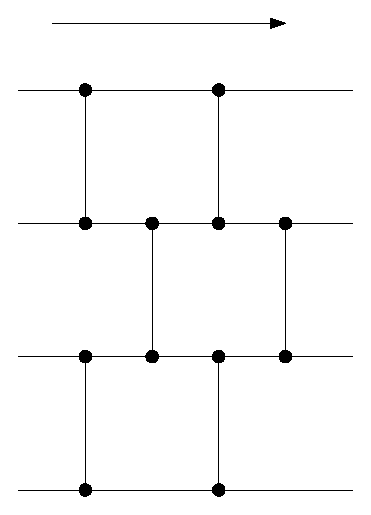
\includegraphics[scale=0.8]{bild2Komparatornetzwerk.eps}
\end{center}
\caption{ } %hier beschreibung
\label{fig:kompnetz2}
% für Referenz nächste Zeil kopieren
% Abbildung \ref{fig:kompnetz2} (Seite \pageref{fig:kompnetz2})
\end{figure}

\begin{figure}
\begin{center}
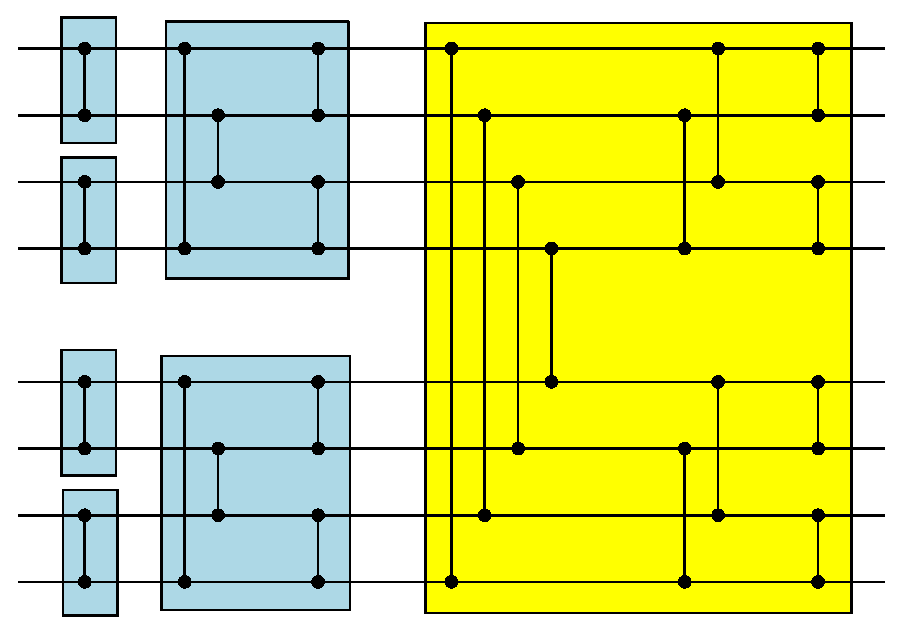
\includegraphics[scale=0.8]{biton1.eps}
\end{center}
\caption{ } %hier beschreibung
\label{fig:biton1}
% für Referenz nächste Zeil kopieren
% Abbildung \ref{fig:biton1} (Seite \pageref{fig:biton1})
\end{figure}

\begin{figure}
\begin{center}
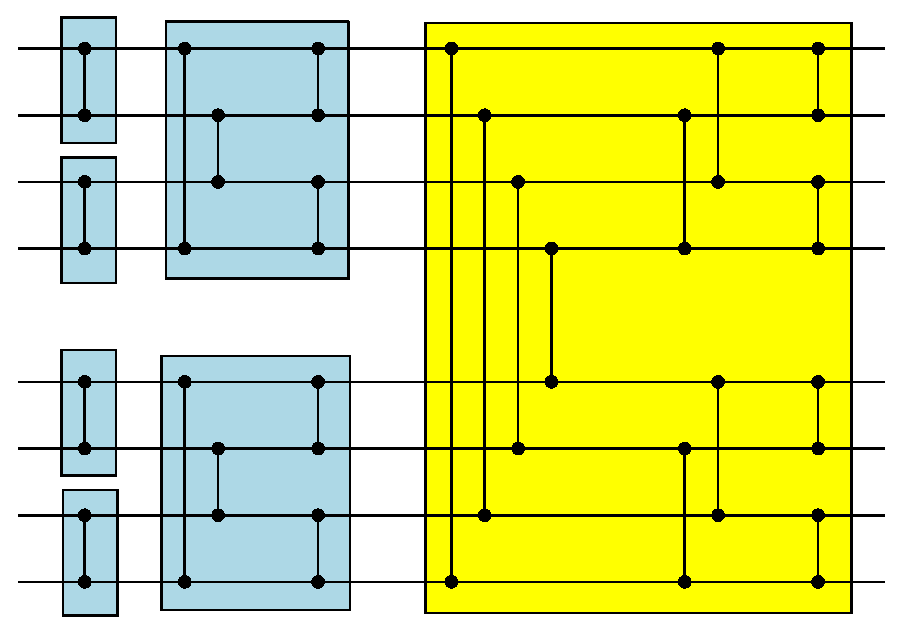
\includegraphics[scale=0.8]{biton2.eps}
\end{center}
\caption{ } %hier beschreibung
\label{fig:biton2}
% für Referenz nächste Zeil kopieren
% Abbildung \ref{fig:biton2 (Seite \pageref{fig:biton2)
\end{figure}

\begin{figure}
\begin{center}
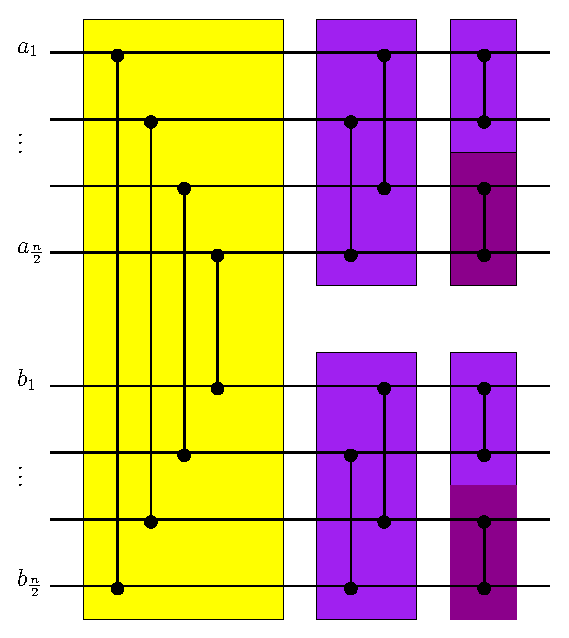
\includegraphics[scale=0.8]{bitonmischer.eps}
\end{center}
\caption{ } %hier beschreibung
\label{fig:bitonmischer}
% für Referenz nächste Zeil kopieren
% Abbildung \ref{fig:bitonmischer} (Seite \pageref{fig:bitonmischer})
\end{figure}